\documentclass[a4paper,11pt,twoside]{article}
\usepackage[T1]{fontenc}
\usepackage{subcaption}
\usepackage[utf8]{inputenc}
\usepackage{ngerman, eucal, mathrsfs, amsfonts, bbm, amsmath, amssymb, stmaryrd,graphicx, array, geometry, color, wrapfig, float, hyperref, epstopdf}
\geometry{left=25mm, right=15mm, bottom=25mm}
\setlength{\parindent}{0em} 
\setlength{\headheight}{0em} 
\title{Machine Learning\\ Blatt 4}
\author{Markus Vieth, David Klopp, Christian Stricker}
\date{\today}
\usepackage{listings, textcomp}
\usepackage[usenames,dvipsnames,svgnames,table]{xcolor}


\definecolor{Code}{rgb}{0,0,0}
\definecolor{Keywords}{rgb}{0,0,255}
\definecolor{Strings}{rgb}{255,0,0}
\colorlet{Comments}{Green}
\colorlet{Numbers}{blue}

%%%%%%%%%%%
%Mache Integer farbig
%%%%%%%%%%%

\makeatletter

\newif\iffirstchar\firstchartrue
\newif\ifstartedbyadigit

\newcommand\processletter
{%
	\ifnum\lst@mode=\lst@Pmode%
	\iffirstchar%
	\global\startedbyadigitfalse%
	\fi
	\global\firstcharfalse%
	\fi
}

\newcommand\processdigit
{%
	\ifnum\lst@mode=\lst@Pmode%
	\iffirstchar%
	\global\startedbyadigittrue%
	\fi
	\global\firstcharfalse%
	\fi
}

\lst@AddToHook{Output}%
{%
	\ifstartedbyadigit%
	\def\lst@thestyle{\color{Numbers}}%
	\fi
	\global\firstchartrue%
	\global\startedbyadigitfalse%
}

\newtoks\jubo@toks
\jubo@toks={
	language=C,
	commentstyle=\color{Comments}\slshape,
	stringstyle=\color{Strings},
	keywordstyle={\color{Keywords}\bfseries},
	alsoletter=0123456789,
	SelectCharTable=%
}
\def\add@savedef#1#2{%
	\begingroup\lccode`?=#1\relax
	\lowercase{\endgroup
		\edef\@temp{%
			\noexpand\lst@DefSaveDef{\number#1}%
			\expandafter\noexpand\csname lsts@?\endcsname{%
				\expandafter\noexpand\csname lsts@?\endcsname\noexpand#2}%
		}}%
		\jubo@toks=\expandafter{\the\expandafter\jubo@toks\@temp}%
	}
	\count@=`0
	\loop
	\add@savedef\count@\processdigit
	\ifnum\count@<`9
	\advance\count@\@ne
	\repeat
	\count@=`A
	\loop
	\add@savedef\count@\processletter
	\ifnum\count@<`Z
	\advance\count@\@ne
	\repeat
	\count@=`a
	\loop
	\add@savedef\count@\processletter
	\ifnum\count@<`z
	\advance\count@\@ne
	\repeat
	%\showthe\jubo@toks % for debugging
	\begingroup\edef\x{\endgroup
		\noexpand\lstdefinestyle{pseudo}{\the\jubo@toks}
	}\x
	
	\makeatother
%%%%%%%%%%
%Ende
%%%%%%%%%%



\lstset{
	literate={ö}{{\"o}}1
	{ä}{{\"a}}1
	{ü}{{\"u}}1
	{ß}{{\ss}}1
	{/pi}{{$\Pi$}}1
	{/inf}{{$\infty$}}1
	{/eIn}{{$\in$}}1
	{/cup}{{$\cup$}}1
	{/leer}{{$\emptyset$}}1
	{<=}{{$\leq$}}1
	{>=}{{$\geq$}}1
}


\lstset{
	numberstyle=\tiny,
	stepnumber=1,
	numbersep=10pt,
	xleftmargin=15pt,
	breaklines=true,
	numberblanklines=false,
	showstringspaces=false,
	flexiblecolumns=true,
	mathescape=true,
	tabsize=4,
	captionpos=b,
	numbers=left,
	commentstyle=\color{Green},
	numberstyle=\color{gray},
	keywordstyle=\color{blue} \textbf,%otherkeywords={xdata},
	keywords=[2]{xdata},
	keywordstyle=[2]\color{red}\textbf,
	identifierstyle=\color{black},
	stringstyle=\color{red}\ttfamily,
	basicstyle = \ttfamily \color{black} \footnotesize,
	inputencoding=utf8,
	emph=[1]%
	{%
		infinity,
	}, 
	emphstyle=[1]{\color{blue}},
	emph=[2]%
	{%
		forall,
		while,
		if,
		else,
		for,
		return,
		new,
		NULL,
		null,
		int, 
		double, 
		float,
		class,
		void,
		false, 
		true,
		FALSE,
		TRUE,
	}, 
	emphstyle=[2]{\color{Magenta}},
	emph=[3]{b0, b1, n0, n1},
	emphstyle=[3]{\color{black}}
}
\begin{document}

\newcommand{\cor}[1]{\textcolor{red}{\textit{#1}}}
\maketitle
\cleardoublepage
\pagestyle{myheadings}
\markboth{Markus Vieth,  David Klopp, Christian Stricker}{Markus Vieth, David Klopp, Christian Stricker}

\newpage

\section*{Nr.1}
\subsection*{b)}
\begin{figure*}[h]
	\captionsetup[subfigure]{labelformat=empty}
	\centering
	\begin{subfigure}[t]{0.33\textwidth}
		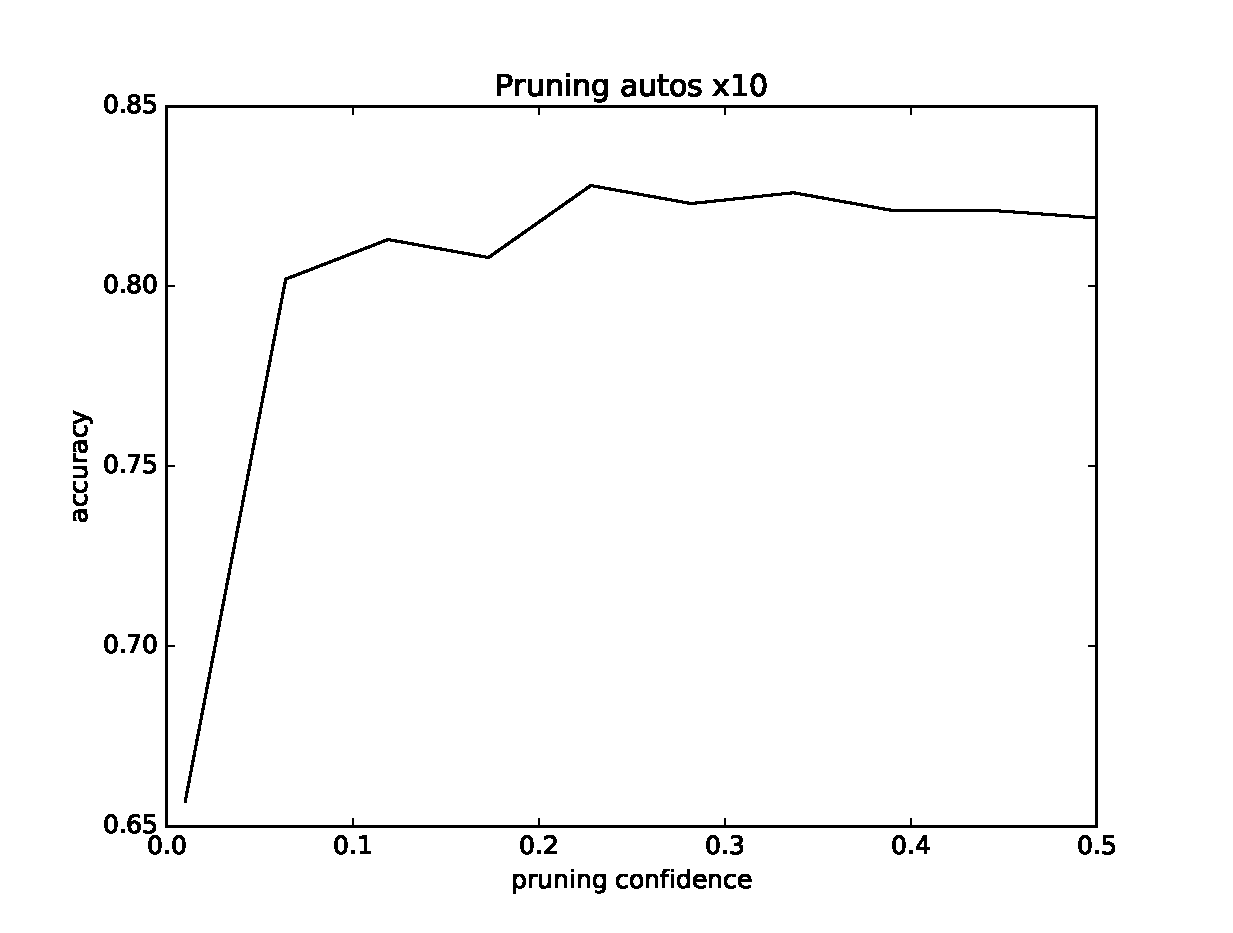
\includegraphics[width=\textwidth]{img/autos.eps}
		\caption{autos dataset}
	\end{subfigure}%
	~
	\begin{subfigure}[t]{0.33\textwidth}
		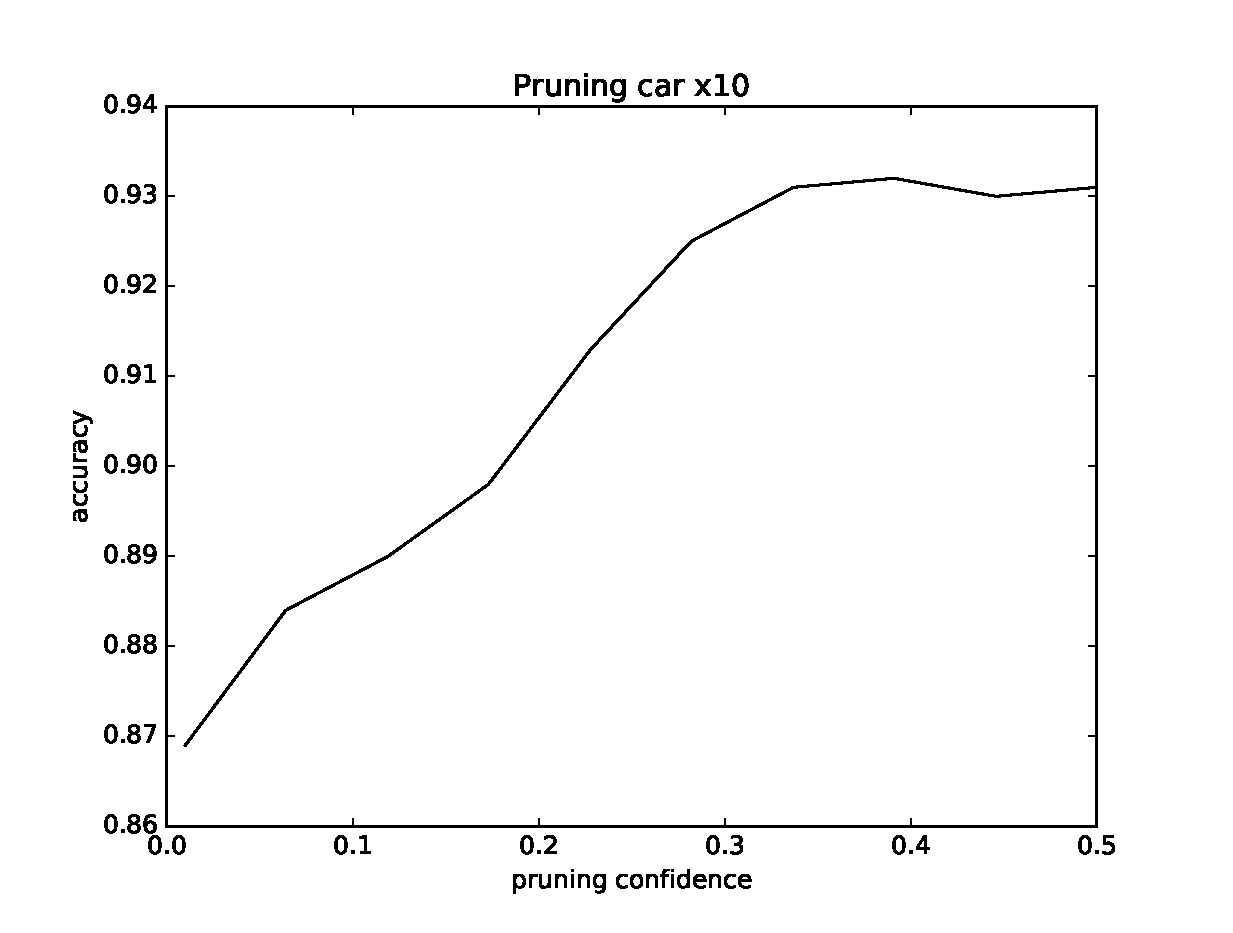
\includegraphics[width=\textwidth]{img/car}
		\caption{car dataset}
	\end{subfigure}%
	~
	\begin{subfigure}[t]{0.33\textwidth}
		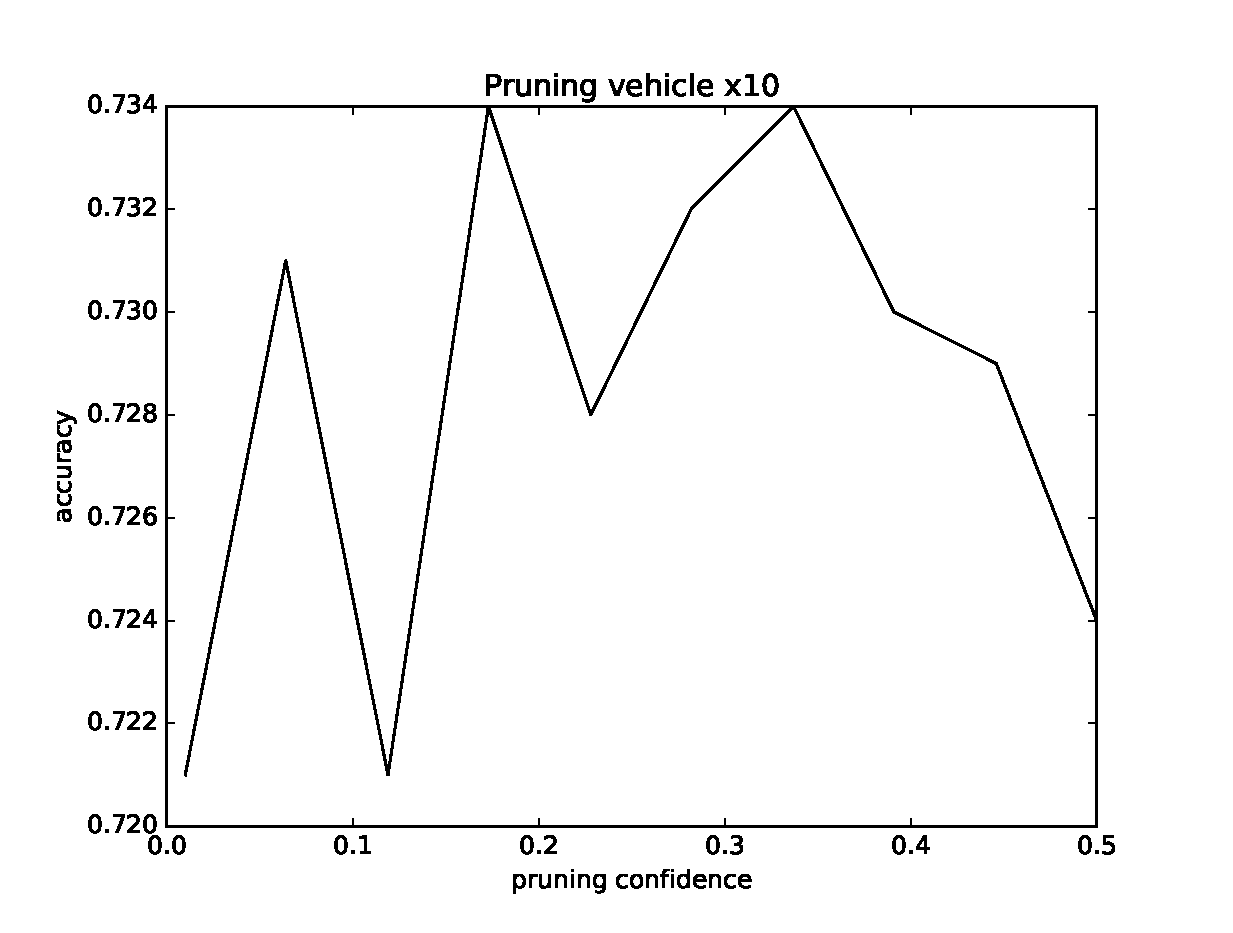
\includegraphics[width=\textwidth]{img/vehicle}
		\caption{vehicle dataset}
	\end{subfigure}
	\caption{Werte wurden über 10 Durchläufe gemittelt}
\end{figure*}
\lstset{language=java}
\subsection*{c)}
\lstinputlisting{OptimalJ48/src/CVParameterSelection.java}
\subsection*{d)}
\lstinputlisting[lastline=96]{OptimalJ48/src/OptimalJ48.java}
\subsection*{e)}
\lstinputlisting[firstline=97]{OptimalJ48/src/OptimalJ48.java}
\subsection*{f)}
\lstinputlisting[lastline=19]{OptimalJ48/src/Test.java}
\lstinputlisting[firstline=22,lastline=24]{OptimalJ48/src/Test.java}
\lstinputlisting[firstline=57,lastline=57]{OptimalJ48/src/Test.java}
\lstinputlisting[firstline=59, lastline=99]{OptimalJ48/src/Test.java}
\subsubsection*{stdout}
Acc aus 10 fold CV über 10 Werte gemittelt. parameter aus CVParameterSelection auf kompletten Datensätzen.\\
\input{OptimalJ48/stdout.txt}
\subsection*{g)}
\lstinputlisting[lastline=19]{OptimalJ48/src/Test.java}
\lstinputlisting[firstline=30,lastline=32]{OptimalJ48/src/Test.java}
\lstinputlisting[firstline=57,lastline=57]{OptimalJ48/src/Test.java}
\lstinputlisting[firstline=124, lastline=134]{OptimalJ48/src/Test.java}
\subsubsection*{stdout}
Acc aus 10 fold CV über 10 Werte gemittelt. parameter aus CVParameterSelection auf kompletten Datensätzen.\\
\input{OptimalJ48/stdout.txt}\\
Gewählte Parameter entsprechen ca. dem lokalen Maximum des Graphen bzw. dem letzten Wert mit Verbesserung.\\
Anmerkung: Kompletter Source-Code in Moodle
\subsection*{h)}
Wie in Aufgabenteil b) zu sehen war, steigt mit der pruning confidence meist auch die accuarcy. Dieses Wachstum stagniert jedoch ab einem bestimmten Punkt. CVParameterSelection wählt nun aus einer vorher festgelegten Menge von Optionen die Werte aus einem angegebenen Intervall, welche die niedrigste error rate aufweisen. Diese wird mithilfe einer n fold CV ermittelt, wobei n eine vorher belegte Variable ist. Da CVParameterSelection die Option nur dann updatet, wenn eine bessere gefunden wurde und die Optionenswerte in steigender Reihenfolge versucht werden, wird der kleinste beste Wert gewählt. Dadurch bleibt das Model (zumindest beim pruning) so einfach wie möglich.
\end{document}